% !TeX spellcheck = fr_FR
\chapter{Chapitre 2 : Notions musicales}
\label{chap:2}

\section{La gamme tempérée}
\label{sec:2.1}

La gamme tempérée ou à tempérament égal est en musique occidentale une gamme qui divise une octave en douze parties sur une échelle logarithmique avec un rapport égal à $\sqrt[12]{2}$. Pour passer à la note suivante, on multiplie la fréquence par $\sqrt[12]{2}$. Et donc inversement, pour passer à la note précédente on divise la fréquence par $\sqrt[12]{2}$.

\begin{figure}[H]
	\centering
	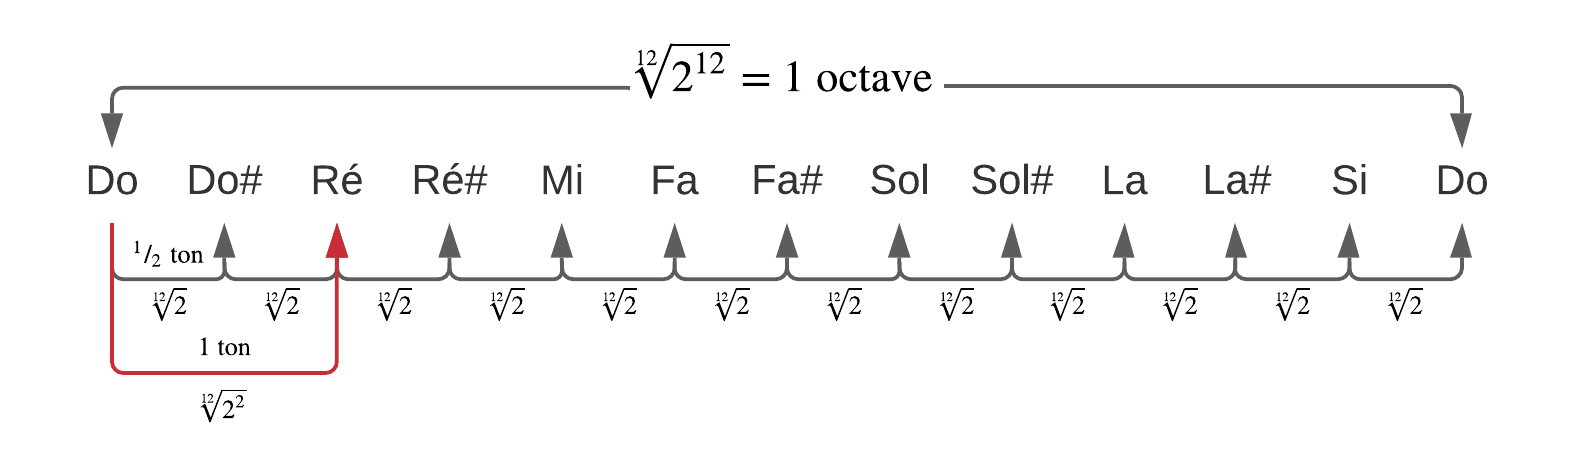
\includegraphics[width=1\linewidth]{gamme_temp}
	\caption[Gamme tempérée]{Gamme tempérée. Source : Réalisé par \textsc{Küenzi} Jean-Daniel}
	\label{fig:gammetemp}
\end{figure}

\section{Les notes de la gamme tempérée}
\label{sec:2.2}

\begin{table}[H]
	\centering{
		\begin{tabular}{|c|c|}
			\hline
			\textbf{Notation anglophone} & \textbf{Notation latine} \\
			\hline
			C & Do \\
			\hline
			C\sh\hspace{2pt}ou D\fl & Do\sh\hspace{2pt}ou Ré\fl \\
			\hline
			D & Ré \\
			\hline
			D\sh\hspace{2pt}ou E\fl & Ré\sh\hspace{2pt}ou Mi\fl \\
			\hline
			E & Mi \\
			\hline
			F & Fa \\
			\hline
			F\sh\hspace{2pt}ou G\fl & Fa\sh\hspace{2pt}ou Sol\fl \\
			\hline
			G & Sol \\
			\hline
			G\sh\hspace{2pt}ou A\fl & Sol\sh\hspace{2pt}ou La\fl \\
			\hline
			A & La \\
			\hline
			A\sh\hspace{2pt}ou B\fl & La\sh\hspace{2pt}ou Si\fl \\
			\hline
			B & Si \\
			\hline 
		\end{tabular}
		\caption[Notes de musique occidentale]{Notes de musiques occidentale. Source : Réalisé par \textsc{Küenzi} Jean-Daniel}
		\label{tab:notes}
	}
\end{table}

Dans cette thèse, nous utiliserons la notation anglophone pour représenter les notes et accords de musique.

\subsection{Explication des dièses (\#) et bémols ($\flat$)}

Dans la musique occidentale, les \# et $\flat$ permettent de représenter les altérations de la hauteur naturelle de la note visée. \# la note est élevée d'un demi-ton, $\flat$ la note est abaissée d'un demi-ton.

\begin{figure}[H]
	\centering
	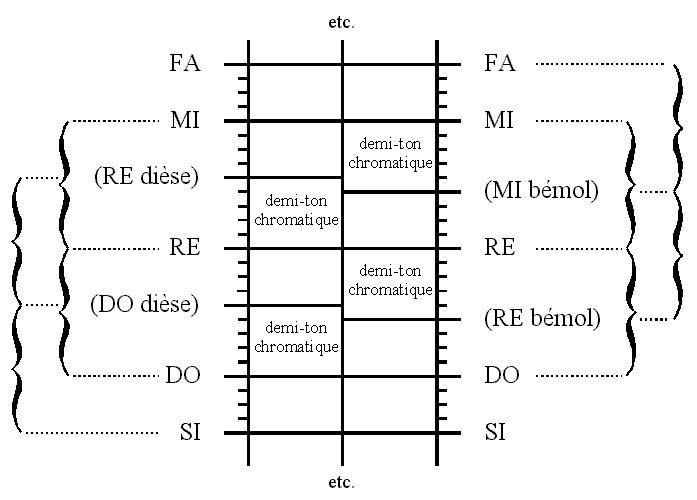
\includegraphics[width=0.7\linewidth]{chroma_ladder}
	\caption[Échelle chromatique]{Échelle chromatique. Source : tiré de \textit{Wikipedia}, ref. URL01}
	\label{fig:chroma_ladder}
\end{figure}

\section{Construction d'un accord à trois sons}
\label{sec:2.3}

En harmonie tonale, un accord à trois sons est composé : d'une fondamentale, d'une tierce qui peut être mineure ou majeure et d'une quinte qui peut être juste, augmentée ou diminuée. Ce qui différencie un accord majeur d'un accord mineur est donc sa tierce.

Dans cette thèse nous verrons uniquement les accords à trois sons dit "parfaits". C'est-à-dire que leur quinte est juste.

\subsection{Majeur}
La construction d'un accord parfait majeur est très simple. Il y a tout d'abord la fondamentale qui va être notre note de base sur laquelle se construit notre accord. Puis la tierce qui est donc majeure, cela veut dire qu'elle se trouve à deux tons de la fondamentale. Puis la quinte qui est juste et se trouve donc à trois tons et demi de la fondamentale.

Prenons comme exemple l'accord AMaj (La Majeur). Il a comme fondamentale A. Puis la tierce majeure qui se trouve à deux tons de la fondamentale, c'est à dire C\sh. Pour finir la quinte juste qui se trouve à trois tons et demi de la fondamentale, c'est à dire E. Notre accord AMaj est donc construit de la manière suivante :

\begin{table}[H]
	\centering{
		\begin{tabular}{|l|c|c|}
			\hline
			\multicolumn{3}{|c|}{\textbf{A Majeur}} \\
			\hline
			& \textbf{Notes} & \textbf{Ton(s)} \\
			\hline
			Fondamentale & A & $\emptyset$ \\
			\hline
			Tierce majeure & C\sh & 2 \\
			\hline
			Quinte juste & E & 3.5 \\
			\hline 
		\end{tabular}
		\caption[Construction de l'accord AMaj]{Construction de l'accord AMaj. Source : Réalisé par \textsc{Küenzi} Jean-Daniel}
		\label{tab:amaj}
	}
\end{table}

\subsection{Mineur}

La construction d'un accord parfait mineur est très simple. Il y a tout d'abord la fondamentale qui va être notre note de base sur laquelle se construit notre accord. Puis la tierce qui est donc mineure. Cela veut dire qu'elle se trouve à un ton et demi de la fondamentale. Puis la quinte qui est juste et se trouve donc à trois tons et demi de la fondamentale.

Prenons comme exemple l'accord Amin (La mineur). Il a comme fondamentale A. Puis la tierce qui doit être mineure et qui se trouve donc à un ton et demi de la fondamentale, c'est à dire C. Pour finir la quinte est juste, elle se trouve donc à trois tons et demi de la fondamentale, c'est à dire E (comme pour AMaj). Notre accord Amin est donc construit de la manière suivante :

\begin{table}[H]
	\centering{
		\begin{tabular}{|l|c|c|}
			\hline
			\multicolumn{3}{|c|}{\textbf{A mineur}} \\
			\hline
			& \textbf{Notes} & \textbf{Ton(s)} \\
			\hline
			Fondamentale & A & $\emptyset$ \\
			\hline
			Tierce mineure & C & 1.5 \\
			\hline
			Quinte juste & E & 3.5 \\
			\hline 
		\end{tabular}
		\caption[Construction de l'accord Amin]{Construction de l'accord Amin. Source : Réalisé par \textsc{Küenzi} Jean-Daniel}
		\label{tab:amin}
	}
\end{table}

\section{Attaque d'une note ou d'un accord}
\label{sec:2.4}

En acoustique, l'attaque est la façon de commencer/jouer une note ou un accord sur un instrument. L'attaque va être un problème dans ce travail, car elle contient beaucoup d'informations (bruit) et se trouve au début de la note, elle va donc fausser l'apprentissage et les résultats prédits. Nous verrons dans le \autoref{chap:4} ce que j'ai mis en place afin d'y pallier.

\section{Transformée de Fourier Discrète (TFD)}
\label{sec:2.5}

La \gls{tfd} sert essentiellement à transformer un signal discret (échantillonné) en une représentation spectrale discrète. L’échantillonnage est fait sur une fenêtre d’analyse bornée dans le temps. La \gls{tfd} va décomposer notre signal en plusieurs superpositions d'ondes sinusoïdales de fréquences différentes. C’est donc un équivalent à la \gls{tf}, mais dans le monde discret et pour les signaux non périodiques. Avec un signal discret $y$ et un nombre d’échantillons $N$, la \gls{tfd} peut être définie comme

{\Large
	\setlength{\abovedisplayskip}{-0.5cm}
	\begin{align*}
			y[k] = \sum_{n=0}^{N-1}{y[n] * \text{exp}(-\frac{2i\pi}{N}kn)} \text{\hspace{10pt}avec 0 $\leq$ k < N}
	\end{align*}
}

\section{Transformée de Fourier Rapide (TFR)}
\label{sec:2.6}

La \gls{tfr} est un algorithme de calculs utilisant la \gls{tfd}. La \gls{tfr} améliore la complexité de la \gls{tfd} $O(N^{2})$, où $N$ est le nombre d’échantillons, en la réduisant à $O(N log N)$ à l’aide de la factorisation matricielle et de divisions du problème en plusieurs parties (diviser pour régner).

\section{Fenêtre de Hamming}
\label{sec:2.7}

Lorsque nous voulons analyser un signal avec une \gls{tfd} ou une \gls{tfr}, on devrait théoriquement connaitre la période du signal que l'on veut analyser. En pratique on ne connait pas toujours cette période. La fenêtre va nous être utile pour éviter la fuite spectrale. La fuite spectrale est un phénomène qui survient lorsque l'on passe à la \gls{tfd} un signal avec une période incomplète. Par exemple pour le A à 220[Hz], examinons son spectre de Fourier sans utiliser une fenêtre de Hamming.

\begin{figure}[H]
	\centering
	\includegraphics[width=1\linewidth]{fft_a220_no_hamming}
	\caption[Spectre de Fourier d'un A à 220 Hertz (fuite spectrale)]{Spectre de Fourier d'un A à 220[Hz] (Fuite spectrale). Source : Réalisé par \textsc{Küenzi} Jean-Daniel}
	\label{fig:fft_a220_no_hamming}
\end{figure}

Comme on peut le voir, la \gls{tfr} nous montre que notre signal est composé de plusieurs sinus autour de 220[Hz]. Or ce n'est pas très juste, même si en pratique il y a toujours du bruit et des interférences, on s'attendrait plutôt à obtenir un spectre plus précis, surtout autour de la fréquence fondamentale. C'est là que la fenêtre de Hamming va nous aider. En multipliant notre signal par cette fenêtre, nous allons réduire la fuite spectrale. Toutefois, on ne peut que la réduire et non l'annuler. Avec un signal $x$, un nombre d'échantillons $N$, la fenêtre de Hamming peut être définie comme

{\Large
	\setlength{\abovedisplayskip}{-0.5cm}
	\begin{align*}
		x[n] = 0.54 - 0.46 \cos(2\pi\frac{n}{N})
	\end{align*}
}

\begin{figure}[H]
	\centering
	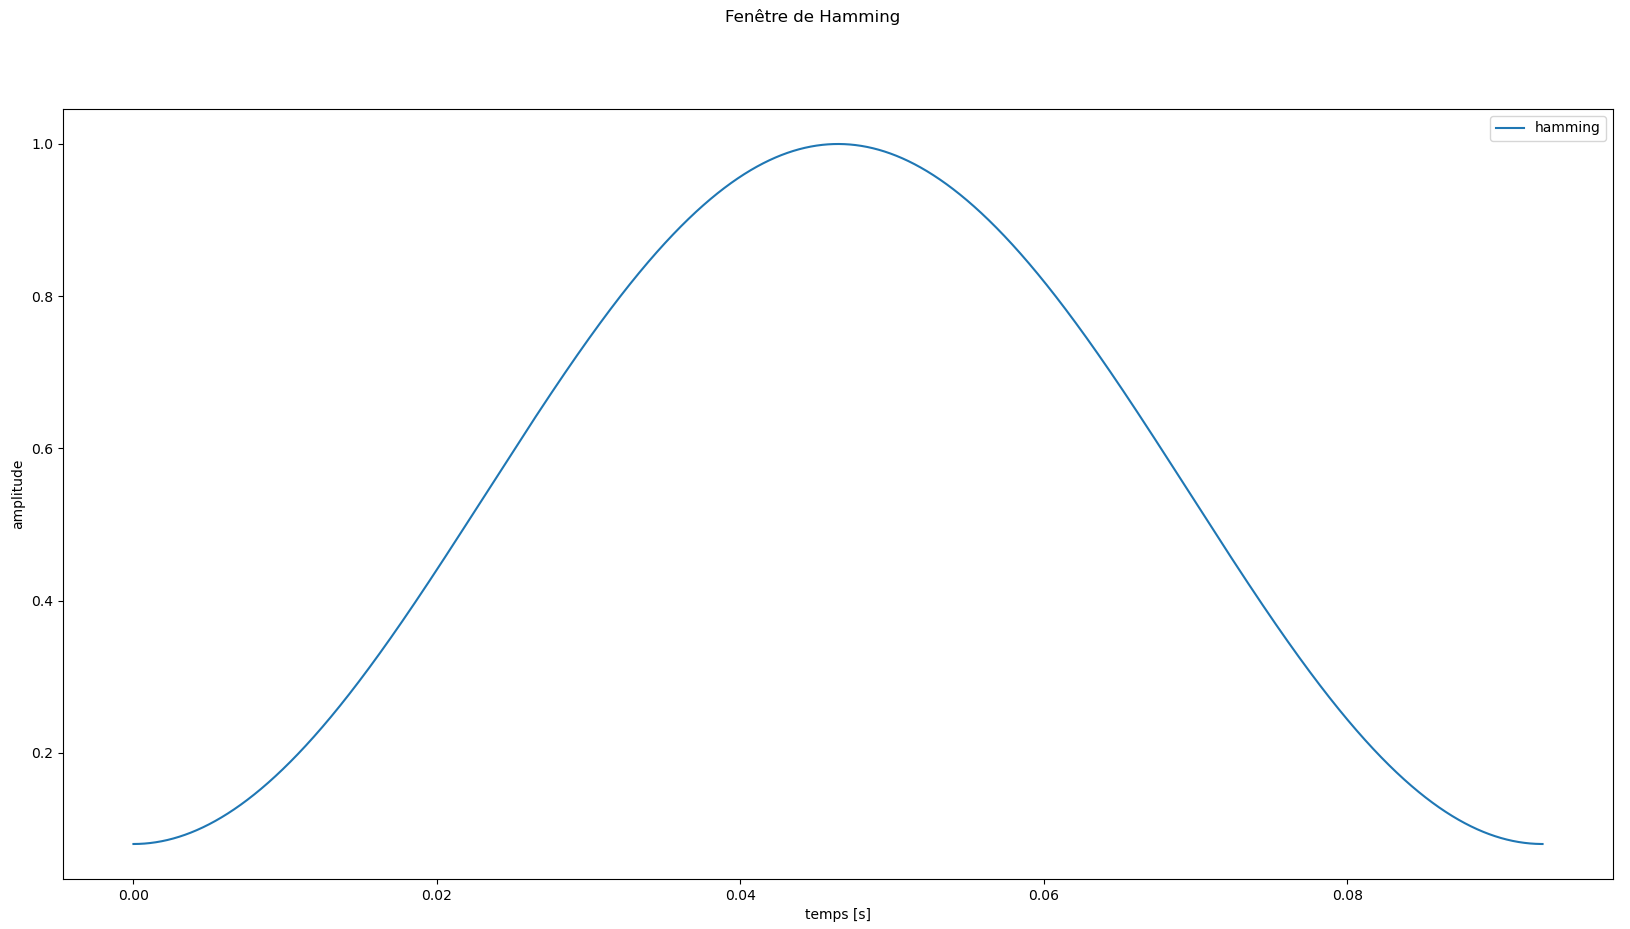
\includegraphics[width=1\linewidth]{hamming_window}
	\caption[Fenêtre de Hamming]{Fenêtre de Hamming. Source : Réalisé par \textsc{Küenzi} Jean-Daniel}
	\label{fig:hamming_window}
\end{figure}

\section{Partiel harmonique}
\label{sec:2.8}

"En acoustique, un partiel harmonique est une composante d’un son périodique, dont la fréquence est un multiple entier d'une fréquence fondamentale." \parencite{noauthor_harmonique_2021}. On peut visualiser les partiels harmoniques d'un signal en affichant son spectre de Fourier. Mais comme la \gls{tfd} se passe dans le monde des nombres complexes, ce que l'on va tracer sur notre spectre est le module de ses nombres. Avec un nombre complexe $z$, la partie réelle $a$ et la partie imaginaire $b$, le module peut être décrit comme

{\Large
	\setlength{\abovedisplayskip}{-0.5cm}
	\begin{align*}
		\lvert z\rvert = \sqrt{a^2 + b^2}
	\end{align*}
}

\subsection{Partiels harmoniques d'une note}

Par exemple pour un A à 220 [Hz] qui est échantillonné à 44.1[kHz] sur une fenêtre de 4096 échantillons, ce qui correspond à une résolution temporelle de \textasciitilde0.093[s], si l'on analyse son spectre de Fourier à l’aide d’une \gls{tfr}, on obtient le spectre suivant

\begin{figure}[H]
	\centering
	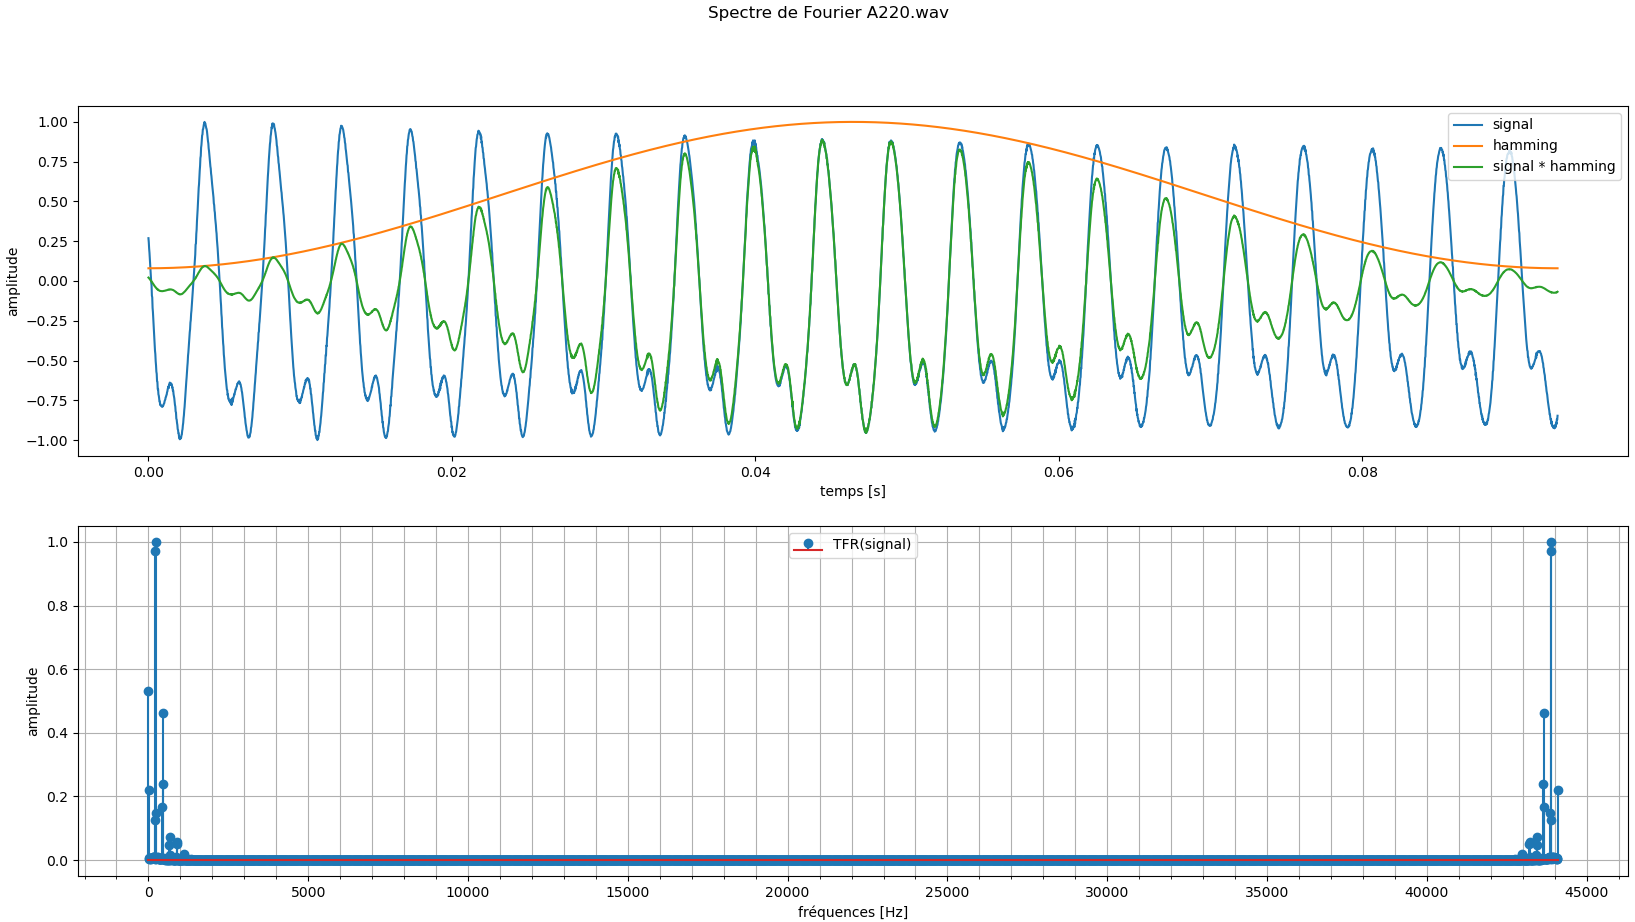
\includegraphics[width=1\linewidth]{fft_total_A220}
	\caption[Spectre de Fourier d'un A à 220 Hertz (entier)]{Spectre de Fourier d'un A à 220[Hz] (entier). Source : Réalisé par \textsc{Küenzi} Jean-Daniel}
	\label{fig:fft_total_a220}
\end{figure}

On ne voit pas grand-chose, mais on peut remarquer tout de même une sorte de symétrie. En fait les fréquences qui se trouvent à droite sont appelées les conjugués des coefficients de Fourier et elles se trouvent après la fréquence de Nyquist. La fréquence de Nyquist est égale à la moitié de la fréquence d'échantillonnage, donc dans notre cas 22.05[kHz]. Mais ce qui nous intéresse est le spectre continu du signal, c'est-à-dire la partie avec les fréquences à gauche. On va donc observer ce qui se passe entre la bande de fréquences [0;1'000] Hertz.

\begin{figure}[H]
	\centering
	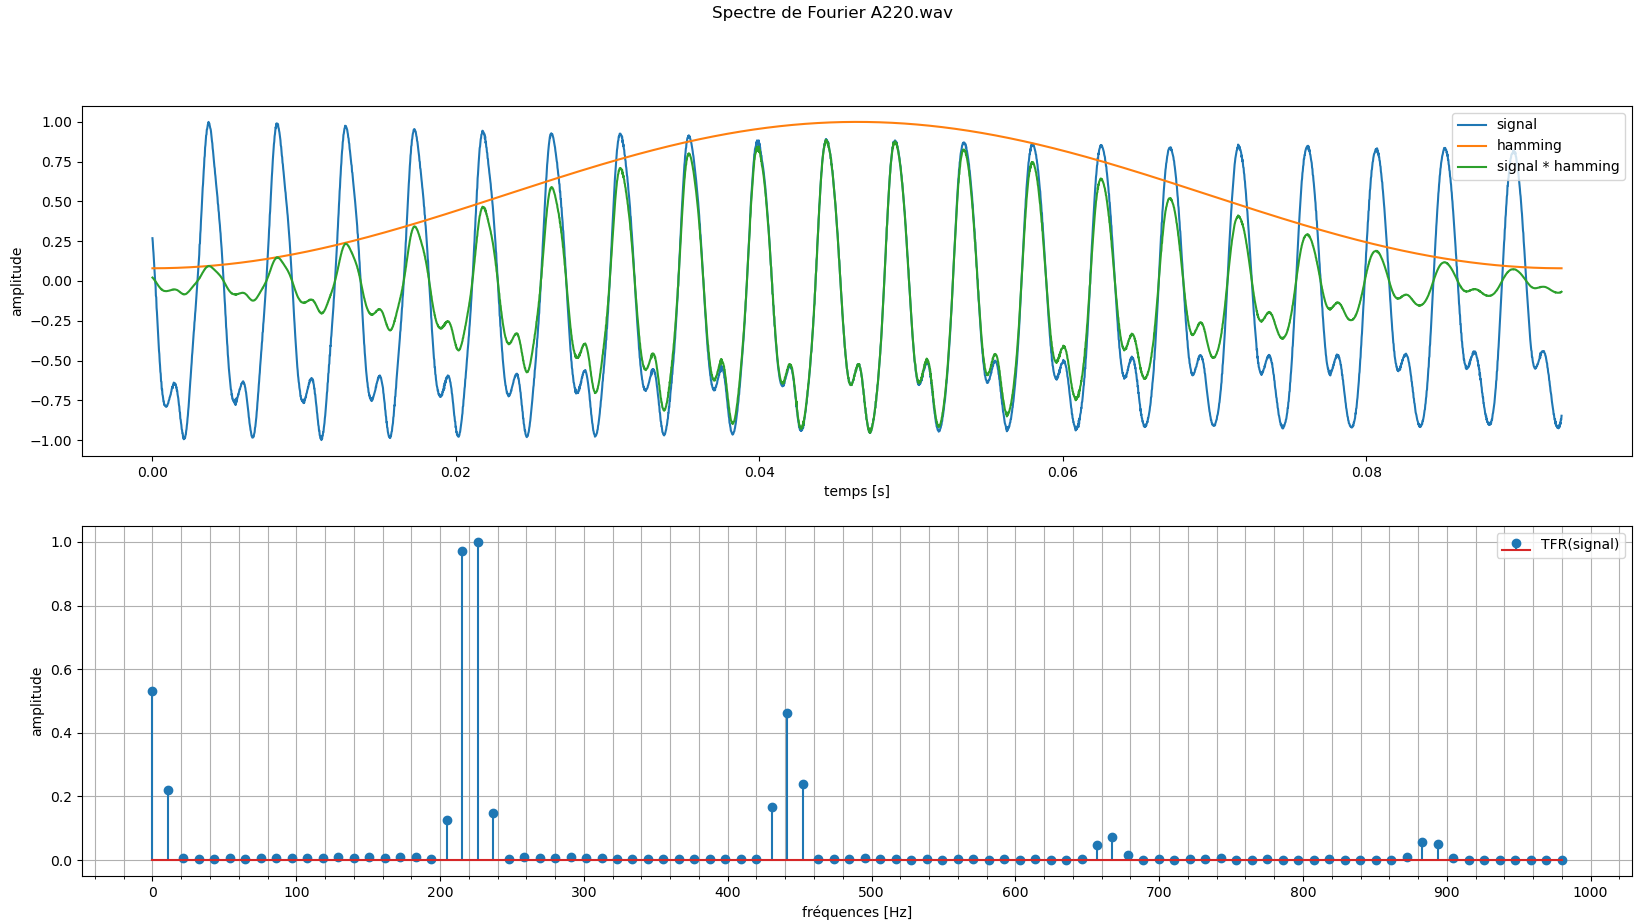
\includegraphics[width=1\linewidth]{fft_A220}
	\caption[Spectre de Fourier d'un A à 220 Hertz (spectre continu)]{Spectre de Fourier d'un A à 220[Hz] (spectre continu). Source : Réalisé par \textsc{Küenzi} Jean-Daniel}
	\label{fig:fft_a220}
\end{figure}

On remarque tout d'abord un pic à zéro. Ce pic correspond à ce qu'on appelle la fréquence nulle. Ensuite, on voit qu’il y a deux pics autour de 220[Hz], ce qui correspond donc à notre fréquence fondamentale, puis un autre pic à 440[Hz] qui correspond donc au premier partiel harmonique $2f_{1}$, puis un troisième à $3f_{1}$, etc. Le spectre de Fourier n'est pas très précis, mais cela s'explique par le fait que nous avons une résolution fréquentielle (précision) de \textasciitilde$10.77$[Hz]. Avec $f_{e}$ la fréquence d'échantillonnage et $n$ la taille de notre fenêtre, la résolution fréquentielle peut être définie comme

{\Large
	\setlength{\abovedisplayskip}{-0.5cm}
	\begin{align*}
		r_f = \frac{f_e}{n}
	\end{align*}
}

\subsection{Partiels harmoniques d'un accord}

Prenons comme exemple un Amin avec comme fondamentale un A à 220[Hz]. Son spectre de Fourier est le suivant :

\begin{figure}[H]
	\centering
	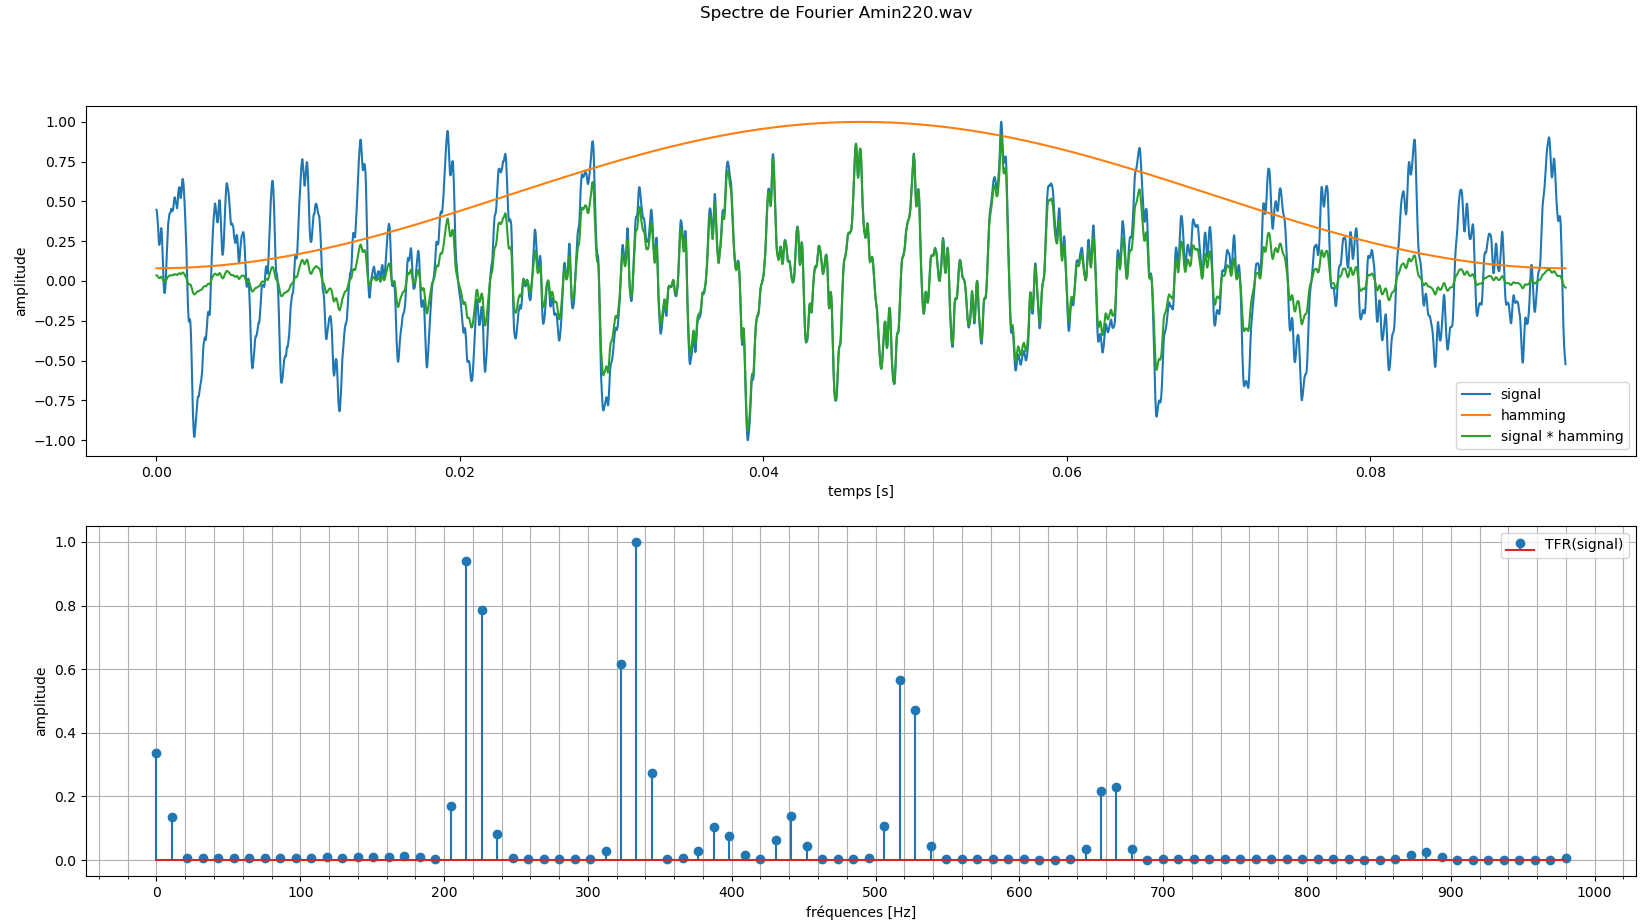
\includegraphics[width=1\linewidth]{fft_Amin220}
	\caption[Spectre de Fourier d'un Amin à 220 Hertz]{Spectre de Fourier d'un Amin à 220[Hz]. Source : Réalisé par \textsc{Küenzi} Jean-Daniel}
	\label{fig:fft_amin220}
\end{figure}

On peut remarquer que le spectre de Fourier contient beaucoup plus de pics que le précédent, ce qui est normal étant donné que notre accord est une superposition de plusieurs notes et donc signaux différents. Mais on remarque bien que nous avons le pic de la fondamentale à \textasciitilde220[Hz] ainsi que ses multiples. Ensuite, on constate un autre pic autour de 330[Hz]. Cela correspond à la quinte E, puis le pic de la tierce C autour de 520[Hz].

On peut se demander pourquoi la tierce a une fréquence plus élevée que la quinte, alors que normalement le C devrait être autour de 260[Hz]. C'est parce que généralement à la guitare on joue la tierce une octave plus haut.
